\section{Scanchain architecture}
\label{sec:scanchain_arch}
%TinyTapeout started as an experiment in fitting as many designs as possible into the 10 mm2 available on the Google lottery shuttles. As a fast proof of concept, a scan chain was chosen. Each design had 8 inputs and 8 outputs. Clock and reset were optional and not treated specially. The chain was formed of scan flops[13], a type of flip flop with an integrated multiplexer at its input.
%
%
%Figure shows 500 designs connected in a chain for TT01, with the scan chain driver in the lower left corner. A dense power distribution network was needed for so many small designs.
%
%
%Figure shows a simplified view of 2 designs in the chain.
%
%
%Each design sends data into the scan flops secondary input and receives input from the output of the flop via a latch. The chain is built[14] by sending data from the output of the previous scan flop into the next scan flops’s primary input.
%
%
%This arrangement allows the loading of data into any of the designs, and then capturing the output and clocking that through the rest of the chain to the output.
%
%
%While relatively easy to implement, the downside is the latency. The more designs in the chain, the longer it takes to send and receive data.
%
%
%Assuming a 50MHz scan chain clock, 250 designs with 8 inputs and 8 outputs, the maximum refresh rate is 50M / (8 * 250) = 25kHz.
%
%
%Another concern is hold violations due to the large number of serially connected flops and potentially large clock skews due to long signal wires. This was mitigated by:
%
%
%* Reclocking the output data with a negedge flop, providing more hold margin
%* Driving the latch and scan signals separately, and with a configurable delay,
%* Keeping wires between designs short by snaking them through the grid.
%
%
%To further reduce the risk of failure, 3 independent methods of driving the chain are provided:
%
%
%1. External - all the signals are available as GPIO pins on the chip. This safest option is the default.
%2. Internal - an internal scan chain driver runs the chain and copies the data to and from 16 GPIOs.
%3. Logic analyser. The Caravel[15] harness provided by Efabless contains a RISCV co-processor with a firmware driven logic analyser. The logic analyser was connected as a 3rd possible way to drive the chain and hence access all designs from firmware.
%
%
%After static timing analysis (STA) it was discovered that the clock duty cycle would increase slightly at each of the 500 sequential clock drivers. This is because P MOSFETs are weaker than N MOSFETs, so for a balanced drive the P MOSFET needs to be substantially larger than the N. To save space, the P mosfet is typically undersized in standard cells, and so the rising clock edge is always slightly slower. This effect limits the maximum clock speed as eventually the clock duty cycle tends to 100%, but faster speeds are possible by starting with a lower duty cycle. With a 50% duty cycle a 30MHz maximum clock is expected, limiting the refresh rate to 7kHz.
%
%
%Alternative:
%
%
%After static timing analysis (STA) it was discovered that the clock duty cycle could change substantially due to the 500 sequential clock drivers. Depending on the exact capacitance between each design, the clock duty cycle could either increase or decrease, with this effect magnified over the chain.
%
%
%TT01’s scan chain was embedded into each design, which created the risk that a user could unintentionally break it, and break the rest of the chain. This risk was mitigated by formally[16] proving the chain was present in the submitted design. For TT02 and TT03, the scan chain was separated into a separate macro block that the user can’t modify.
%
%
%Figure showing TT02 designs with separate scan chain blocks.
%
%
%For TT01 and TT02 each design used 2 clock buffers, with the internal flops driven after the first buffer.
%
%
%TT03 used inverting clock buffers, with only one between clock in and out.
%
%
%This meant that the clock is inverted between each design, so the delay caused by the P MOSFETs were evenly spread across the negative and positive cycles. With this change the chain should be able to be driven up to around 60MHz, for an update frequency of 30kHz.
%
%
%The verification[17] effort was broad and included a community review, register transfer level (RTL) and gate level (GL) simulation, Formal Verification[18], static timing analysis, layout vs schematic (LVS), DRC and device level static verification[19].

TinyTapeout started as an experiment in fitting as many designs as possible into the \(10 mm^2\) available on the Google lottery shuttles.
As a fast proof of concept, a scan chain was chosen.
Each design had 8 inputs and 8 outputs.
Clock and reset were optional and not treated specially. The chain was formed of scan flops\cite{skywaterpdk}, a type of flip flop with an integrated multiplexer at its input.

\begin{figure}[htp]
\centering
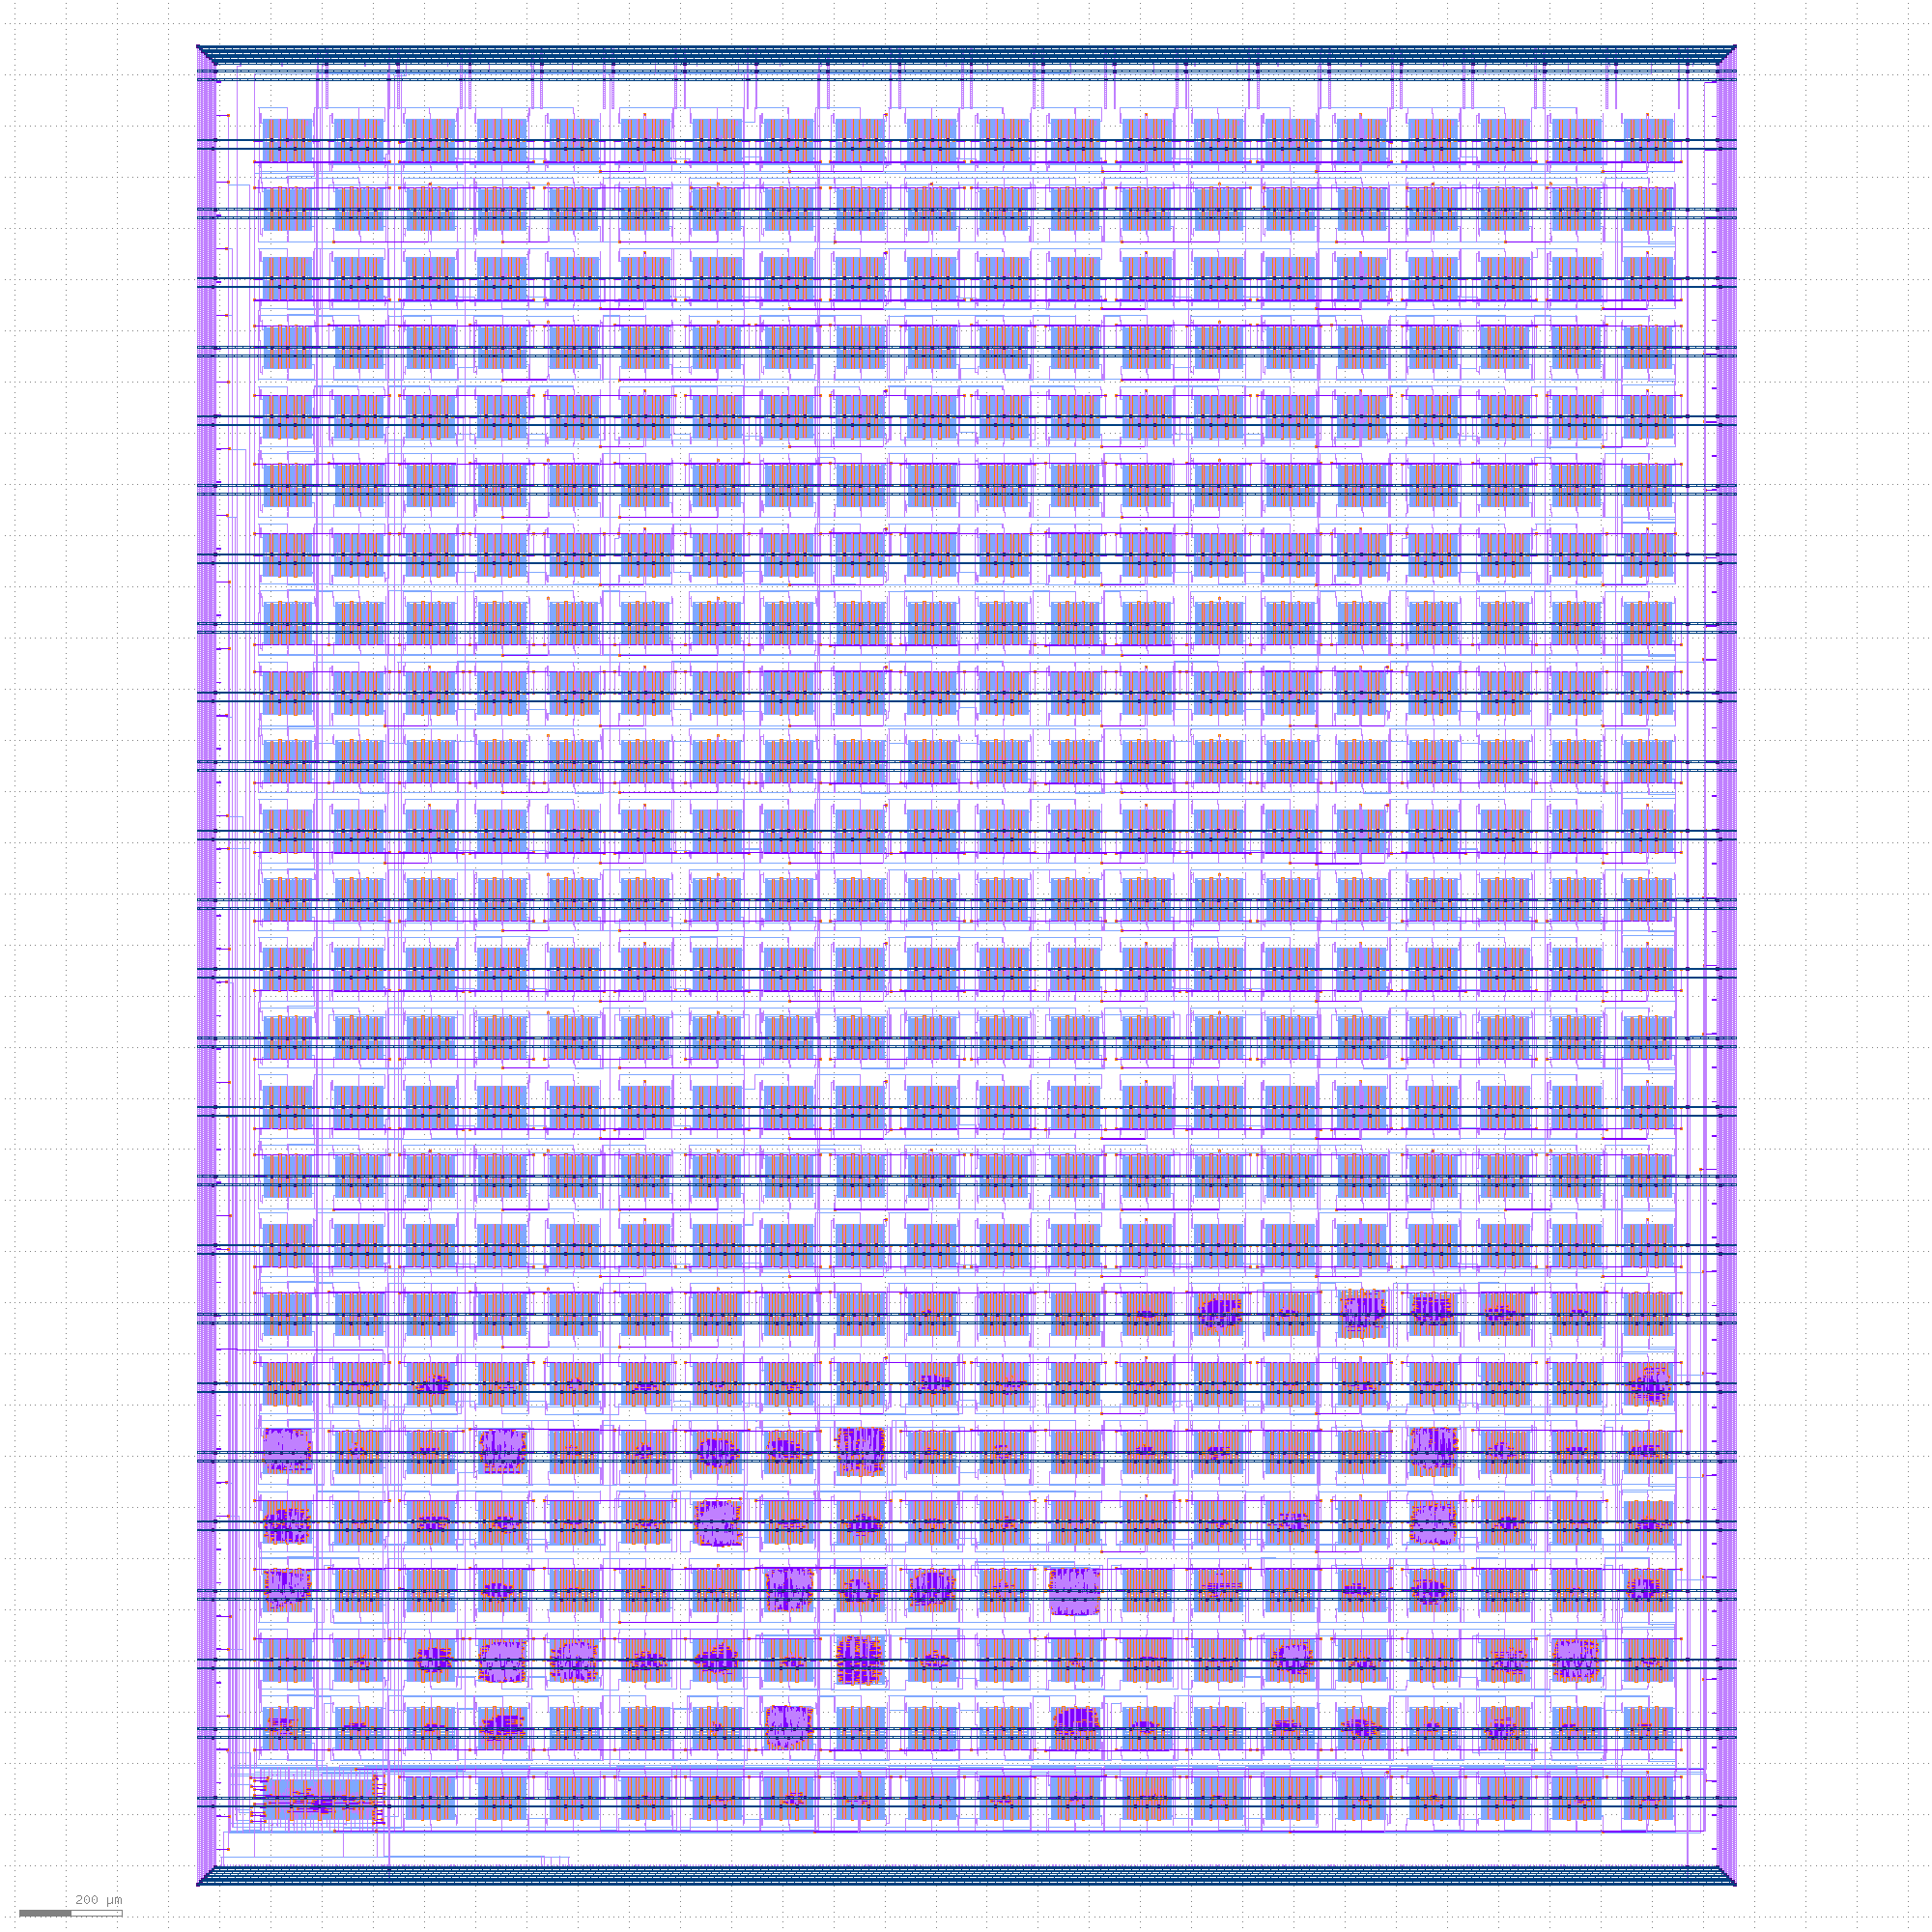
\includegraphics[width=1\columnwidth]{./Figs/tt01_whole_die.png}
\caption{500 designs connected in a chain for TT01, with the scan chain driver in the lower left corner.}
\label{fig:500_designs_chain_TT01}
\end{figure}

\begin{figure}[htp]
\centering
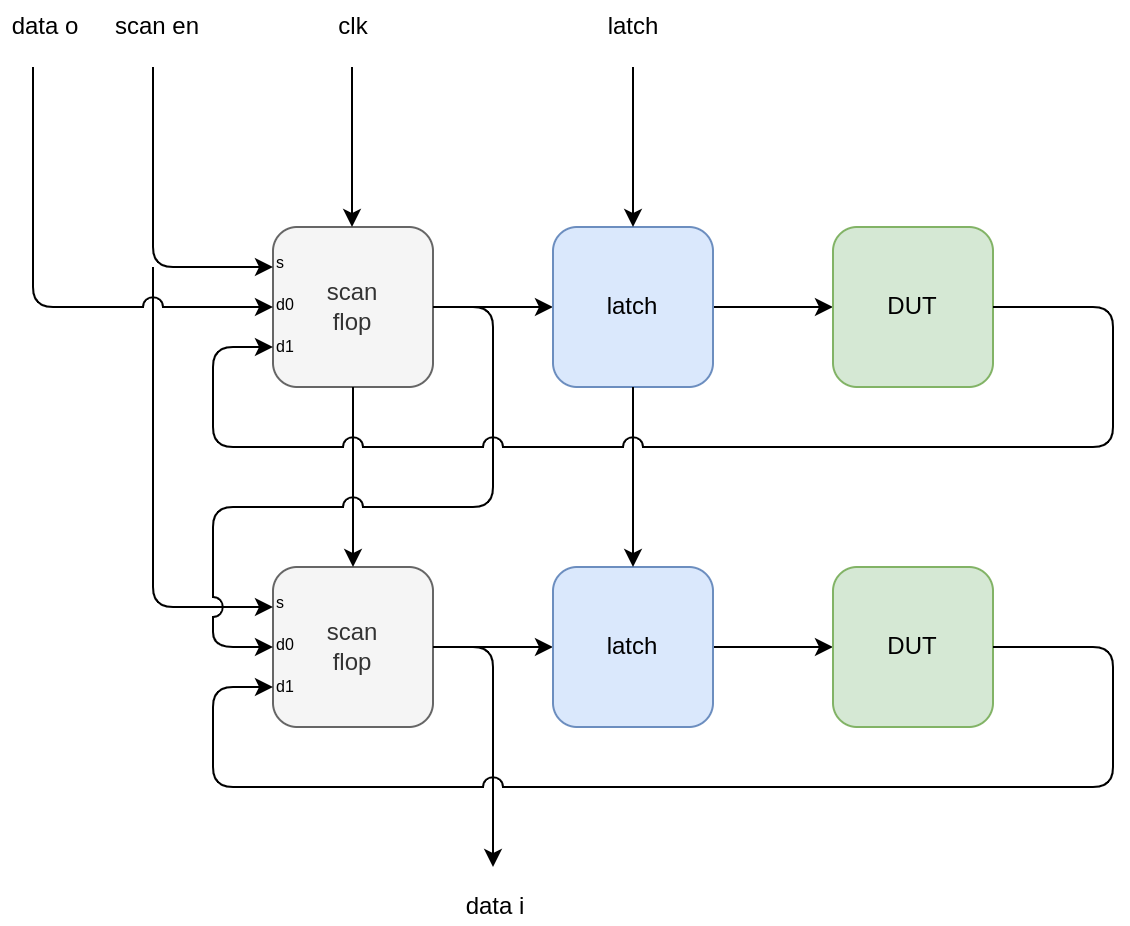
\includegraphics[width=\columnwidth]{./Figs/scanchain_block_diagram.png}
\caption{A simplified view of 2 designs in the chain.}
\label{fig:simplified_view_2_designs}
\end{figure}

Each design sends data into the scan flops secondary input and receives input from the output of the flop via a latch.
The chain is built\cite{updateiodesign} by sending data from the output of the previous scan flop into the next scan flops’s primary input.

This arrangement allows the loading of data into any of the designs, and then capturing the output and clocking that through the rest of the chain to the output.

While relatively easy to implement, the downside is the latency.
The more designs in the chain, the longer it takes to send and receive data.

Assuming a \(50 MHz\) scan chain clock, \(250\) designs with \(8\) inputs and \(8\) outputs, the maximum refresh rate is \(50M / (8 \times 250) = 25kHz\).

Another concern is hold violations due to the large number of serially connected flops and potentially large clock skews due to long signal wires.
This was mitigated by:
\begin{itemize}
\item Reclocking the output data with a negedge flop, providing more hold margin.
\item Driving the latch and scan signals separately, and with a configurable delay.
\item Keeping wires between designs short by snaking them through the grid.
\end{itemize}

To further reduce the risk of failure, three independent methods of driving the chain are provided:
\begin{enumerate}
\item External - all the signals are available as GPIO pins on the chip. This safest option is the default.
\item Internal - an internal scan chain driver runs the chain and copies the data to and from \(16\) GPIOs.
\item Logic analyser - The Caravel\cite{caravel} harness provided by Efabless contains a RISC-V co-processor with a firmware driven logic analyser. The logic analyser was connected as a third possible way to drive the chain and hence access all designs from firmware.
\end{enumerate}

After static timing analysis (STA) it was discovered that the clock duty cycle would increase slightly at each of the \(500\) sequential clock drivers.
This is because PMOS transistors are weaker than NMOS transistors, so for a balanced drive the PMOS needs to be substantially larger than the NMOS.
To save space, the PMOS is typically undersized in standard cells, and so the rising clock edge is always slightly slower. This effect limits the maximum clock speed as eventually the clock duty cycle tends to \(100\%\), but faster speeds are possible by starting with a lower duty cycle. With a \(50\%\) duty cycle a \(30 MHz\) maximum clock is expected, limiting the refresh rate to \(7 kHz\).

TT01’s scan chain was embedded into each design, which created the risk that a user could unintentionally break it, and break the rest of the chain.
This risk was mitigated by formally\cite{tinytapeoutscan} proving the chain was present in the submitted design.
For TT02 and TT03, the scan chain was separated into a separate macro block that the user can’t modify.

\begin{figure}[htp]
\centering
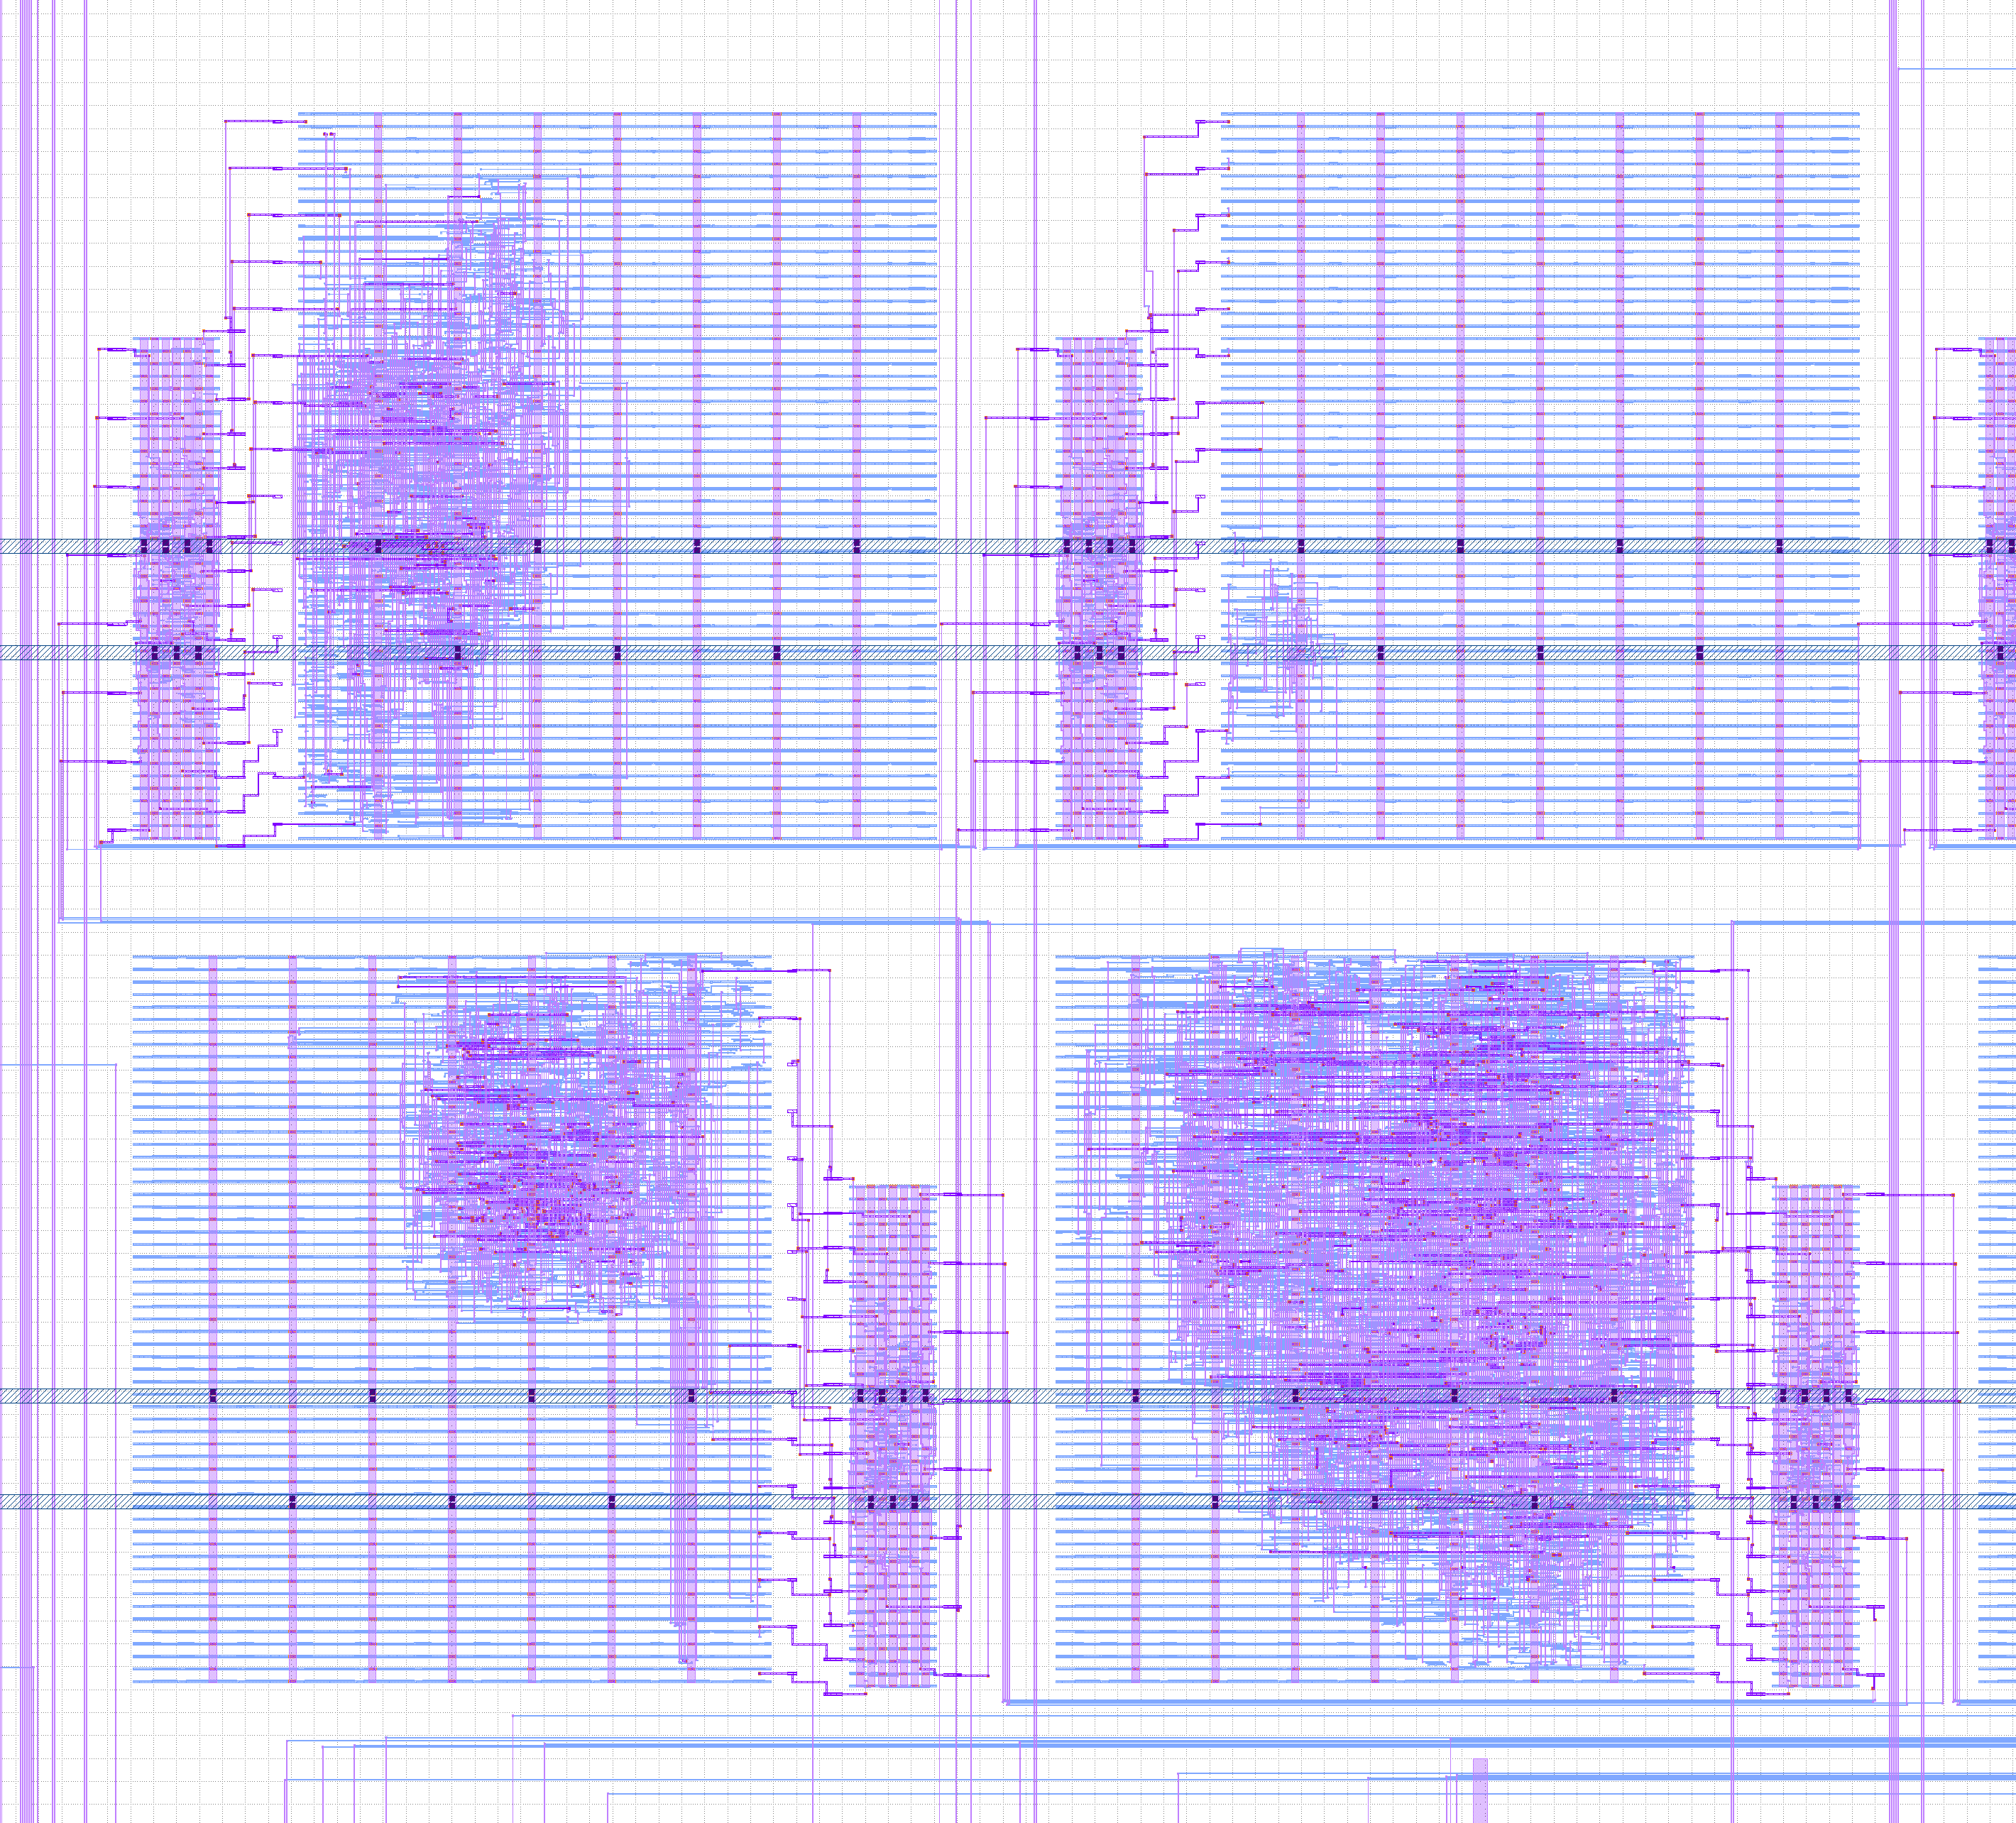
\includegraphics[width=\columnwidth]{./Figs/tt02_gds_zoom.png}
\caption{TT02 designs with separate scan chain blocks.}
\label{fig:TT02_separate_scan_blocks}
\end{figure}

\begin{figure}[htp]
\centering
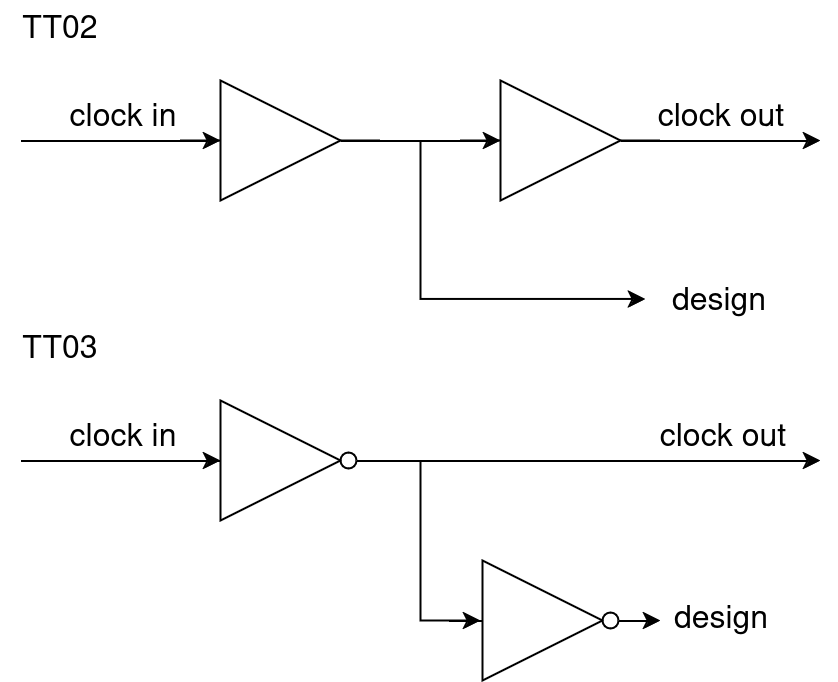
\includegraphics[width=\columnwidth]{./Figs/tt02 vs tt03 scanchain clock.png}
\caption{Differences between TT02 and TT03 scanchain clock buffers.}
\label{fig:TT02_vs_TT03}
\end{figure}

For TT01 and TT02 each design used two clock buffers, with the internal flops driven after the first buffer.

TT03 used inverting clock buffers, with only one between the clock in and out.

This meant that the clock is inverted between each design, so the delay caused by the PMOS transistors were evenly spread across the negative and positive cycles.
With this change, the chain should be able to be driven up to around \(60 MHz\), for an update frequency of \(30 kHz\).

The verification effort\cite{verificationmd} was broad and included a community review, register transfer level (RTL) and gate level (GL) simulation, Formal Verification\cite{sby}, static timing analysis, layout vs schematic (LVS), DRC, and device level static verification\cite{cvc}.
